\documentclass[a4paper]{exam}

\usepackage{amsmath,amssymb, amsthm}
\usepackage{geometry}
\usepackage{graphicx}
\usepackage{hyperref}
\usepackage{xcolor}
\usepackage{wasysym}

\usepackage{xcolor}
\usepackage{wasysym}


\usepackage{tikz}
\usepackage{tikz-qtree}

\usetikzlibrary{automata, positioning, arrows}
\tikzset{
  ->,  % makes the edges directed
  >=stealth, % makes the arrow heads bold
  node distance=2cm, % specifies the minimum distance between two nodes. 
  every state/.style={thick, fill=gray!10}, % sets the properties for each ’state’ node
  initial text=$ $, % sets the text that appears on the start arrow 
}
% Header and footer.
\pagestyle{headandfoot}
\runningheadrule
\runningfootrule
\runningheader{CS 212}{HW 1: Regular Languages}{Fall 2024}
\runningfooter{}{Page \thepage\ of \numpages}{}
\firstpageheader{}{}{}


\newcommand{\shuffle}{\textsc{shuffle}} % Use \shuffle typeset this operator.
\newcommand{\cut}{\textsc{cut}} % Use \cut typeset this operator.
\newcommand{\complexcut}{\textsc{complex-cut}} % Use \complex-cut typeset this operator.


\newtheorem{definition}{Definition}
\newtheorem{theorem}{Theorem}

\title{Homework 1: Regular Languages: Automata and Expressions}
\author{CS 212 Nature of Computation\\Habib University}
\date{Fall 2025}

\boxedpoints


% \printanswers % Uncomment this line

\begin{document}
\maketitle


\begin{questions}
    \question[10]
    \begin{definition}[Power on a language]
        Given a language $L$, we define $L^n$, for $n \in \mathbb{N}$ recursively as follows:
        \begin{enumerate}
            \item $L^0 = \{\varepsilon\}$ 
            \item $L^1 = L$
            \item $L^{k+1} = \{w_1w_2\mid w_1 \in L^k \land w_2 \in L\}$
        \end{enumerate}
    \end{definition}
    \begin{definition}[Kleene closure]
        With this definition of $L^n$, we can define Kleene closure of $L$, $L^*$ as follows:
        $$L^*=\bigcup_{i \in \mathbb{N}} L^i$$
    \end{definition}
    \begin{definition}[Positive closure]
        With this definition of $L^n$, we can define Positive closure of $L$, $L^+$ as follows:
        $$L^+=\bigcup_{i \in \mathbb{Z}^+} L^i$$
    \end{definition}
    
    Let $L \subseteq \Sigma^*$ be a language. Prove or disprove the following claim:
    $(L^+)^*=(L^*)^+$
    
    \begin{solution}
        % Enter your solution here.
    \end{solution}
    
    \textbf{Note:} $\mathbb{N}$ here denotes the set of natural numbers which includes 0. See \href{https://en.wikipedia.org/wiki/Set-theoretic_definition_of_natural_numbers}{von Neumann ordinals} for the construction of $\mathbb{N}$.
    $\mathbb{Z}^+$ denotes the set of positive integers.

    \titledquestion{title}[10]

    \begin{definition}[Shuffle Operator]
        Let $L \subseteq \{0,1\}^*$ be a some language. The operator $\shuffle$ is defined as, $\shuffle(L) = \{w\in \{0,1\}^*\mid \exists x \in L \;s.t. \; w \text{ is obtained by shuffling the characters of } x\}$. More formally, $\shuffle(L) = \{w = w_1w_2\dots w_n\in \{0,1\}^*\mid \exists x = x_1x_2 \dots x_n \in L, \;s.t.\; \forall w_i !\exists x_j : w_i = x_j\}$. 
    \end{definition}
    
    Prove or disprove the following claim: 
    If $L$ is a regular language then $\shuffle(L)$ is also regular.
    (You can not assume the pumping lemma in this problem.)

    \begin{solution}
        % Enter your solution here.
    \end{solution}

    \question After failing to make it big with your CS degree from Habib university, you tried to try your luck with gambling. 
    You notice that at poker tables to avoid cheating decks are ``cut'' before the round starts. 
    The traditional method for cutting a deck of playing cards, the deck is arbitrarily split two parts, which are exchanged before reassembling the deck.
    But you can never be too careful with card cheats, for this you see people using a more complex method for cutting the deck in which the deck is broken into three parts and the middle part in placed first in the reassembly.
    But your brain is broken after taking CS212 in fall 2025, and all you can think about are regular languages. You wonder if regular languages can be cut like that. With the mathematical skills you obtained from the course you were able to come up with the following formalism for the two types of cuts.
    $$\cut(L) = \{w_2w_1 \in \Sigma^*\mid w_1w_2 \in L, \text{ where each } w_i \text{ is some string in } \Sigma^*\}$$
    $$\complexcut(L) = \{w_2w_1w_3 \in \Sigma^*\mid w_1w_2w_3 \in L, \text{ where each } w_i \text{ is some string in } \Sigma^*\}$$

    Where $L$ is some language. Now realizing that you have already lost all your life savings, you shift your focus on more important matters and start to wonder if regular languages are closed under these operators that you defined.

    \begin{parts}
        \part[10] Prove or disprove the following claim: The class of regular language is closed under $\cut$ operation.
          \begin{solution}
            % Enter your solution here.
          \end{solution}

        \part[10] Prove or disprove the following claim: The class of regular language is closed under $\complexcut$ operation.
          \begin{solution}
            % Enter your solution here.
          \end{solution}

    \end{parts}

    \begin{center}
        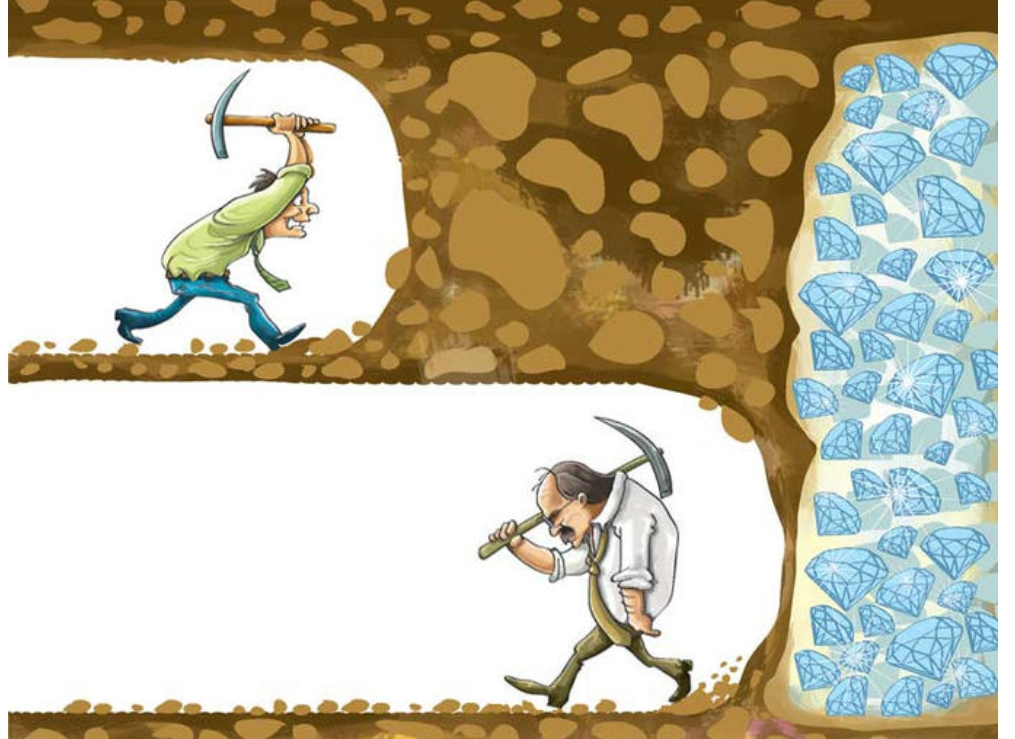
\includegraphics[scale = 0.25]{keep_gambling.png}
    \end{center}
    
  
  
\end{questions}

\end{document}

%%% Local Variables:
%%% mode: latex
%%% TeX-master: t
%%% End:



